%%% In this section, you will describe all of the various artifacts that you will generate and maintain during the project life cycle. Describe the purpose of each item below, how the content will be generated, where it will be stored, how often it will be updated, etc. Replace the default text for each section with your own description. Reword this paragraph as appropriate.

\subsection{Major Documentation Deliverables}
These deliverables are major grade components of the course. Completing these documents should generally be the sprint goal during the applicable sprint period. Remove this paragraph from your draft, but leave the heading.

\subsubsection{Project Charter}
Describe how this document will be maintained and updated (how often, under what circumstances, etc.). When will the initial version be delivered? When will the final version be delivered?

\subsubsection{System Requirements Specification}
Describe how this document will be maintained and updated (how often, under what circumstances, etc.). When will the initial version be delivered? When will the final version be delivered?

\subsubsection{Architectural Design Specification}
Describe how this document will be maintained and updated (how often, under what circumstances, etc.). When will the initial version be delivered? When will the final version be delivered?

\subsubsection{Detailed Design Specification}
Describe how this document will be maintained and updated (how often, under what circumstances, etc.). When will the initial version be delivered? When will the final version be delivered?

\subsection{Recurring Sprint Items}
The following items will be documented and maintained during each individual sprint. Remove this paragraph from your draft, but leave the heading.

\subsubsection{Product Backlog}
How will items be added to the product backlog from the SRS? How will these items be prioritized? Who makes the decision (product owner, group vote, etc.)? What software will be used to maintain and share the product backlog with team members and stakeholders?

\subsubsection{Sprint Planning}
How will each sprint plan be planned? How many sprints will there be (you need to look at the schedules for this course and previous Senior Design II courses during the appropriate semesters to figure this out).

\subsubsection{Sprint Goal}
The spring goal will decided by the group. We will discuss what a reasonable goal will be based on our knowledge and the difficulty of the task. The input from the customer will also be taken in consideration.

\subsubsection{Sprint Backlog}
The team leader will decided what backlog products will make into the sprint backlog. The backlog will be maintained by the team leader in a shared file in Google Drive or GitHub.


\subsubsection{Task Breakdown}
Each individual from the team will list their programming skills and based on that will be given a task to complete. The amount of time that they have to complete will be documented in the sprint as well, also if they find a task that they think it fits their set of skill, they can claim that task for themselves.

\subsubsection{Sprint Burn Down Charts}
Who will be responsible for generating the burn down charts for each sprint? How will they be able to access the total amount of effort expended by each individual team member? What format will the burn down chart use (include an example burn down chart below).

\begin{figure}[h!]
    \centering
    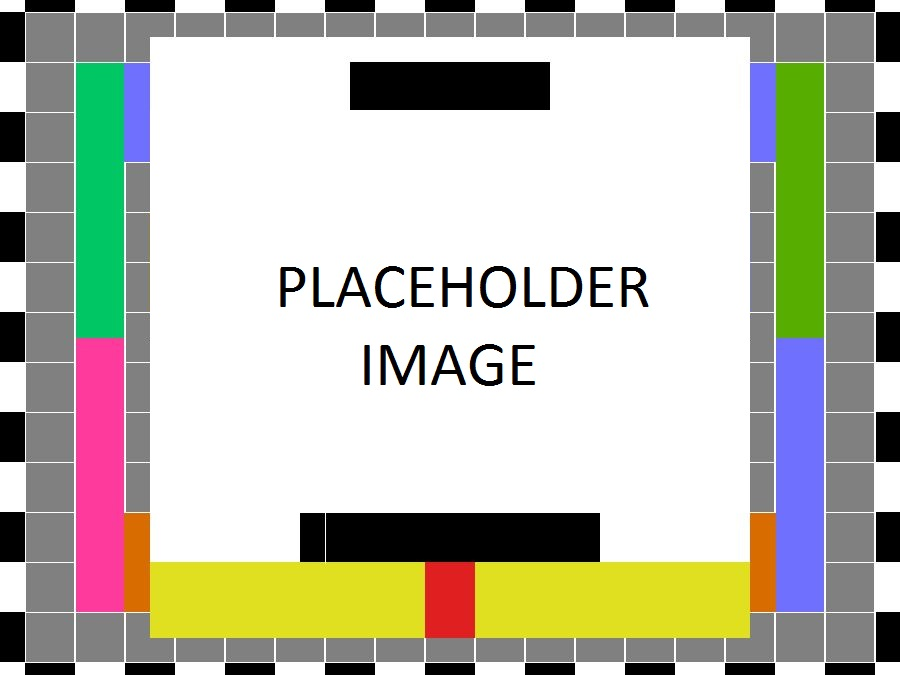
\includegraphics[width=0.5\textwidth]{images/test_image}
    \caption{Example sprint burn down chart}
\end{figure}

\subsubsection{Sprint Retrospective}
How will the sprint retrospective be handled as a team? When will this discussion happen after each sprint? What will be documented as a group and as individuals, and when will it be due?

\subsubsection{Individual Status Reports}
What sort of status will be reported by each individual member, and how often will it be reported? What key items will be contained in the report?

\subsubsection{Engineering Notebooks}
How often will the engineering notebook be updated, at a minimum, by each team member? What is the minimum amount of pages that will be completed for each interval, and how long will that interval be? How will the team keep each member accountable? Who will sign of as a "witness" for each ENB page?



\subsection{Closeout Materials}
The following materials, in addition to major documentation deliverables, will be provided to the customer upon project closeout. Remove this paragraph from your draft, but leave the heading.

\subsubsection{System Prototype}
What will be included in the final system prototype? How and when will this be demonstrated? Will there be a Prototype Acceptance Test (PAT) with your customer? Will anything be demonstrated off-site? If so, will there be a Field Acceptance Test (FAT)?

\subsubsection{Project Poster}
What will be included on the poster, what will be the final dimensions, and when will it be delivered?

\subsubsection{Web Page}
What will be included on the project web page? Will it be accessible to the public? When will this be delivered? Will it be updated throughout the project, or just provided at closeout (at a minimum, you need to provide a simple web page at the end).

\subsubsection{Demo Video}
The demo video will include a brief demonstration of the computer screen and smart phone applications working together as well one of our members working with the scanner and label maker. The approximated time will be about 2 - 4 minutes. The topics covered will be the label making, scanning a new product, managing the database from the desktop application.

\subsubsection{Source Code}
The source code will be maintained in GitHub. Both the source code and the executable files will be provided to the customer. All of there will be saved in a cloud service so that it can be downloaded as many times is needed. The source code will be posted in a public repository in GitHub for the general public with a MIT license. The license will be listed in the "read-me" file or its own file.

\subsubsection{Source Code Documentation}
What documentation standards will be employed? Will you use tools to generate the documentation (Doxygen, Javadocs, etc.). In what format will the final documentation be provided (PDF, browsable HTML, etc.)?

The documentation will be done using Doxygen and a PDF will be provided to the customer.

\subsubsection{Hardware Schematics}
Project is only software.

\subsubsection{CAD files}
Project is only software.

\subsubsection{Installation Scripts}
The mobile application will be sent through GitHub and installed in the device via Android Studio. If any desktop application is developed, it will be provided using a installation script. 

\subsubsection{User Manual}
The customer will be provided with a digital manual and there will also be instructions in the application as well. If the software proves to be more complicated that we think, then a setup video will be created to show the customer how to operate the software and hardware.